\documentclass[twoside,11pt]{article}
\usepackage{jmlr2e}
\usepackage{amsmath}
\usepackage{booktabs}
\usepackage{graphicx}
\usepackage{lastpage}
\usepackage{tabularx}
\usepackage{url}
\hypersetup{hidelinks}
\setlength{\textfloatsep}{7pt plus 2pt minus 2pt}
\setlength{\floatsep}{6pt plus 2pt minus 2pt}
\setlength{\intextsep}{6pt plus 2pt minus 2pt}
\setlength{\abovecaptionskip}{3pt}
\setlength{\belowcaptionskip}{0pt}
\renewcommand{\arraystretch}{0.96}

\jmlrheading{1}{2026}{1--\pageref{LastPage}}{7/26}{}{26-0000}{Kassim et al.}
\ShortHeadings{kodama-cpp}{Kassim et al.}
\firstpageno{1}

\begin{document}

\title{kodama-cpp: Cross-Validated Accuracy Maximization on CPU, CUDA, and Apple Metal}

\author{%
\name Moussa Kassim$^{1,2,\ast}$ \email moussa.kassim@icgeb.org\\
\name Martin Ocharo$^{1,2,\ast}$ \email martin.ocharo@icgeb.org\\
\name Dalia Ahmed$^{1}$ \email dalia.ahmed@icgeb.org\\
\name Dupe Ojo$^{1}$ \email dupe.ojo@icgeb.org\\
\name Alessia Vignoli$^{3,4}$ \email vignoli@cerm.unifi.it\\
\name Leonardo Tenori$^{3,4,\dagger}$ \email tenori@cerm.unifi.it\\
\name Stefano Cacciatore$^{1,2,\dagger}$ \email stefano.cacciatore@icgeb.org\\
\addr $^1$Bioinformatics Unit, International Centre for Genetic Engineering and Biotechnology (ICGEB), Cape Town 7925, South Africa\\
\addr $^2$Department of Integrative Biomedical Sciences, Institute of Infectious Disease \& Molecular Medicine (IDM), University of Cape Town, Cape Town 7925, South Africa\\
\addr $^3$Department of Chemistry ``Ugo Schiff'', University of Florence, Sesto Fiorentino, Italy\\
\addr $^4$Magnetic Resonance Center (CERM), University of Florence, Sesto Fiorentino, Italy\\
\addr $^{\ast}$Moussa Kassim and Martin Ocharo contributed equally.\\
\addr $^{\dagger}$Leonardo Tenori and Stefano Cacciatore are co-corresponding authors.}

\editor{To be assigned}
\maketitle

\begin{abstract}
KODAMA discovers latent structure by maximizing held-out label predictability. This standalone C++17 implementation is shared by thin R and Python wrappers. Native multicore CPU, NVIDIA CUDA, and Apple Metal backends provide float32 KNN and SIMPLS--LDA without silent fallback. The library also introduces prediction-guided label evolution and exact-quota landmark projection. Tests distinguish numerical consistency and systems performance from external-label diagnostics.
\end{abstract}

\begin{keywords}
KODAMA, cross-validation, unsupervised learning, heterogeneous computing, manifold learning
\end{keywords}

\section{Introduction}

KODAMA treats labels as optimization variables: useful labels can be reproduced on held-out samples. An ensemble of optimized vectors then corrects neighborhood dissimilarities \citep{cacciatore2014kodama,cacciatore2017kodama}. Unlike stability analysis or prediction strength, predictability is inside the search and no observed labels anchor it \citep{benhur2002stability,tibshirani2005predictionstrength}.

Repeated cross-validation makes reusable state a systems concern. Our four contributions are \textbf{(1)} a typed C++ core shared by R and Python; \textbf{(2)} CPU, CUDA, and Metal under one float32 contract; \textbf{(3)} prediction-guided evolution with adaptive proposals, degeneracy guards, and error-scaled cooling; and \textbf{(4)} exact-quota landmark projection, formalizing the principle introduced by \citet{abdelshafy2025landmarks}.

\clearpage
\section{KODAMA objective and algorithm}

For data $X\in\mathbb{R}^{n\times p}$, labels $y$, folds $\Pi$, and classifier family $\mathcal F$, let
\begin{equation}
  A(y;X,\mathcal F,\Pi)=\frac{1}{n}\sum_{i=1}^{n}\mathbf{1}\!\left[y_i=\widehat y_i^{(-\Pi(i))}\right].
\end{equation}
KODAMA searches for high $A$ using either KNN or SIMPLS followed by latent-space LDA \citep{dejong1993simpls}. Folds stay fixed within each run, and supplied constraint groups move atomically. Each independent run draws exactly $L$ landmarks by population-proportional quotas from a coarse matrix partition; randomized systematic rounding fills the residual quota without replacement. A separate partition initializes the labels, so sampling strata are not optimization targets.

The classifiers share an evolution \emph{scaffold}, not an identical state policy. Both use fixed folds, prediction-guided grouped proposals, the common transition matrix, one new CV pass per proposal, error-scaled cooling, and independent $M$ runs. Let $p_k$ be the class proportions, $D=1-\sum_kp_k^2$, $H=-\sum_kp_k\log p_k$, $K_{\rm eff}=e^H$, and $R=\max\{0,\log[K/\max(1,K_{\rm eff})]\}$. State selection uses
\begin{equation}
  S_{\mathcal F}(y)=A(y)\sqrt D-\mathbf{1}_{\{\mathcal F={\rm PLS\mbox{-}LDA}\}}(1-A(y))
  \max\!\left\{\frac{H}{\log n},\frac{R}{1+R}\right\}.
\end{equation}
Standard \texttt{KODAMA.matrix} applies transition-driven coarsening and the subtraction only to PLS--LDA; KNN uses the common diversity term alone. This reflects that LDA fits a mean per active class, whereas KNN has no analogous global class fit. Existing sensitivity results motivate, but do not isolate, this policy; no universal improvement is claimed.

The selected landmark vector is projected to all samples with the same classifier. If $a_{ij}$ is the fraction of projected runs agreeing on graph edge $(i,j)$, KODAMA returns $d'_{ij}=(1+d_{ij})/a_{ij}^{2}$ and removes zero-agreement edges. Exact proposal, temperature, quota, and coarsening formulas are given in the supplement.

\begin{figure}[h!]
\hrule\vspace{2pt}
\begin{minipage}{0.98\linewidth}
\footnotesize
\textbf{Algorithm 1: KODAMA ensemble}\\
\textbf{Input:} $X,\mathcal F,M,T,L,K_0,\Pi,s$.\quad \textbf{Output:} $G,C,A_{\rm best},Z_U,Z_T$.
\begin{tabbing}
\quad\=\quad\=\quad\=\kill
$X_{32}\leftarrow\textsc{Float32}(X)$; $(G_0,Z_U,Z_T)\leftarrow\textsc{KODAMA.Graph}(X_{32})$ once\\
\textbf{for} $r=1,\ldots,M$ \textbf{do}\\
\> $I_r\leftarrow\textsc{ExactQuotaSample}(\textsc{Partition}(X,K_0),L,s+r)$\\
\> $y\leftarrow\textsc{InitialPartition}(X_{I_r},K_0)$; $(A,\widehat y)\leftarrow\textsc{CV}(\mathcal F,X_{I_r},y,\Pi_r)$\\
\> \textbf{for} $t=1,\ldots,T$ \textbf{do}\\
\>\> $y'\leftarrow\textsc{GuidedProposal}(y,\widehat y,t,T)$; if $\mathcal F={\rm PLS\mbox{-}LDA}$, apply transition coarsening\\
\>\> $(A',\widehat y')\leftarrow\textsc{CV}(\mathcal F,X_{I_r},y',\Pi_r)$; update by $S_{\mathcal F}$ and cooling\\
\> \textbf{end for}\\
\> $C_{\cdot r}\leftarrow\textsc{Project}(\mathcal F,X_{I_r},y_{\rm best},X)$\\
\textbf{end for}\\
$G\leftarrow\textsc{AgreementCorrectionInPlace}(G_0,C)$; \textbf{return} $G,C,A_{\rm best},Z_U,Z_T$
\end{tabbing}
\end{minipage}
\vspace{-4pt}\hrule
\caption{Compact pseudocode. The scaffold is common; the indicated coarsening and score term are PLS--LDA-specific.}
\label{alg:kodama}
\end{figure}

\clearpage
\section{Standalone heterogeneous implementation}

\begin{figure}[h!]
\centering
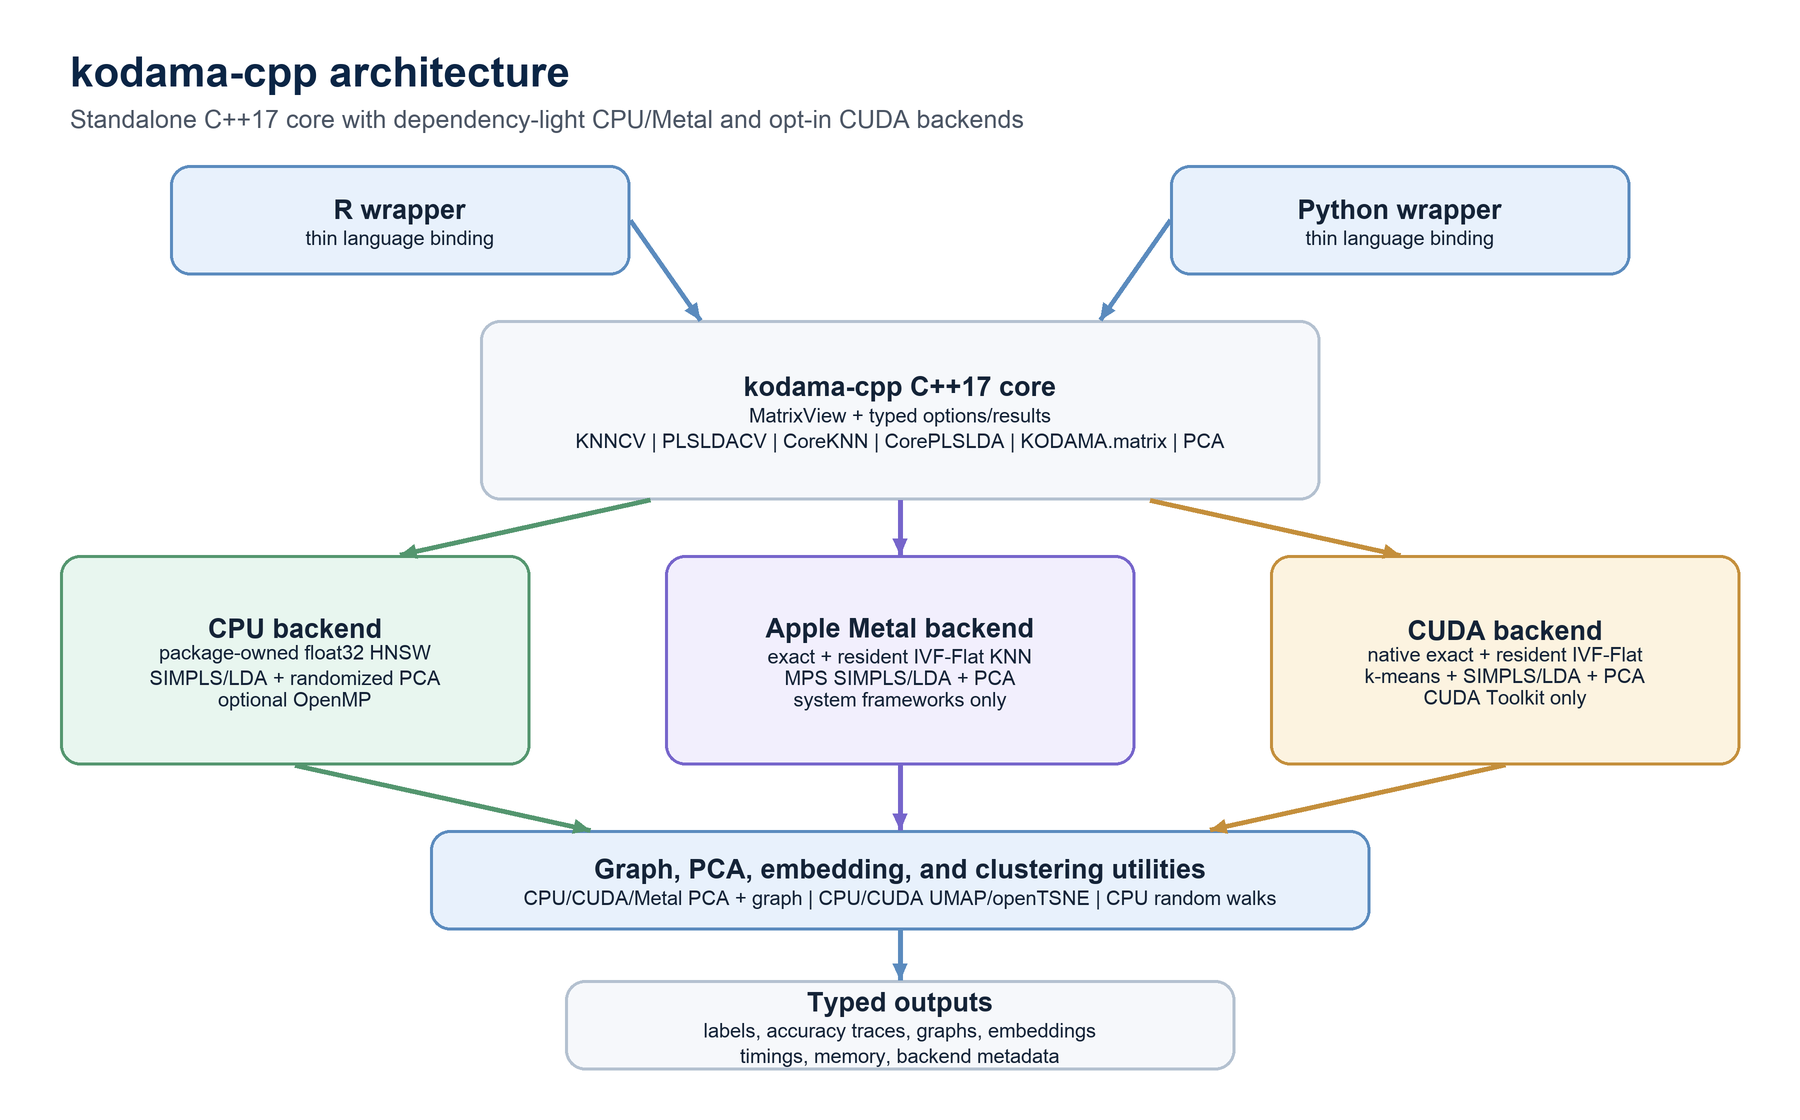
\includegraphics[width=0.68\linewidth]{kodama_cpp_architecture.png}
\caption{The C++17 core owns algorithm state; R and Python are thin adapters. For a fixed classifier, backends share folds, policy, component semantics, and typed results.}
\label{fig:architecture}
\end{figure}

The typed C++ API owns folds, proposals, classifiers, landmark projection, graph correction, and metadata; wrappers only convert host objects and results. CPU supplies parallel HNSW construction over contiguous float32 storage \citep{malkov2020hnsw}, with a deterministic connected base seed before lock-protected concurrent insertion and querying, plus SIMPLS--LDA, PCA, graph operations, and embeddings. CUDA supplies exact/IVF KNN, batched k-means, label-aware SIMPLS--LDA, PCA, and embeddings. Metal supplies exact/IVF KNN, k-means, MPS-assisted SIMPLS--LDA, and PCA. Accelerator IVF construction and persistent indices retain training data and index state on-device. During KODAMA, one resident full-data graph and persistent worker-lane buffers retain fold layouts, labels, projections, voting state, and PLS--LDA workspaces across proposal cycles; contents that depend on a new landmark sample are refreshed in place once per $M$ run. Unsupported backends raise an error rather than silently falling back.

PLS--LDA forms class cross-products without dense one-hot responses, compacts active labels, reuses fold workspaces, and evaluates the requested feasible component count without model selection. \texttt{KODAMA.graph} prepares one full-data neighbor graph and separately scaled backend-matched UMAP/openTSNE PCA starts. Its result owns only graph arrays, starts, and metadata: it never retains the raw matrix. The wrappers reserve \texttt{data} for raw features and \texttt{graph} for a prepared object or bare paired $n\times k$ index/distance graph; either can be supplied alone or both can be supplied together, and raw-only input invokes graph preparation internally. Graph-only execution uses disclosed self-tuning normalized-Laplacian geometry, including the PLS--LDA spectral surrogate, whereas supplying raw features retains ordinary data-input PLS--LDA. Fixed-graph KNN reuses supplied neighborhoods and is distinguished from data-native KNN rather than asserted to reproduce its stochastic trajectory. Final compaction and agreement correction mutate the single graph owner in place. The API also exposes both CV kernels, both core optimizers, PCA, and float32 UMAP/openTSNE \citep{mcinnes2018umap,vandermaaten2008tsne}. Explicit visualization starts take precedence, then backend-matched stored starts, then raw-data recomputation and graph-only fallbacks; provenance is reported. Derivations, safeguards, pseudocode, evidence, and API contracts are in the supplement.

\section{Validation, availability, and scope}

\begin{table}[h!]
\caption{Matched runtime and held-out accuracy. Times are seconds; KODAMA reports median raw CV accuracy for $M=T=100$.}
\label{tab:validation}
\centering\scriptsize
\begin{tabular}{lllrrrr}
\toprule
Scope & Data & Accel. & CPU & Device & Speedup & Accuracy \\
\midrule
KNNCV & MNIST & CUDA & 76.769 & 4.753 & 16.2 & .974/.973 \\
PLSLDACV & MetRef & CUDA & 1.294 & 0.308 & 4.20 & .992/.993 \\
KODAMA PLS--LDA & MetRef & CUDA & 341.648 & 270.408 & 1.26 & .9924/.9924 \\
KNNCV & MetRef & Metal & 11.145 & 0.026 & 425.0 & .827/.827 \\
PLSLDACV & MetRef & Metal & 0.790 & 0.202 & 3.90 & .991/.990 \\
\bottomrule
\end{tabular}
\end{table}

Table~\ref{tab:validation} separates kernels from the complete KODAMA call. CUDA and Metal preserved closely matched held-out accuracy, while end-to-end acceleration was smaller because repeated orchestration and graph work remain. Finite-precision ties may select different stochastic trajectories, so numerical consistency is assessed by contracts and paired metrics rather than bitwise label identity. Extended runtime, memory, landmark, $M/T$, visualization, and prior-version comparisons are reported in the supplement.

The fixed-$M=100$ sensitivity study also shows why classifier-independent scoring is not claimed: at $T=100$, median active-class counts were 9 versus 24 on MetRef and 32 versus 71 on USPS for KNN versus PLS--LDA. These observations establish different fragmentation regimes, but because they are not penalty-on/off ablations they do not establish the causal benefit of the PLS--LDA term.

CTest and wrapper suites exercise float32 numerics, strict backend identity, graph and PCA contracts, backend-matched visualization initialization, landmark counts, and the candidate-\texttt{0.1.0} API. A controlled CPU openTSNE comparison against the pinned fastEmbedR source was coordinate-identical. GitHub Actions covers Linux/macOS CPU, native Metal, wrappers, coverage, and API documentation; CUDA is validated on a dedicated NVIDIA host. The audited CPU snapshot reached 63.58\% line and 57.03\% branch coverage.

The MIT-licensed core is available at \url{https://github.com/tkcaccia/kodama-cpp}; the R wrapper is at \url{https://github.com/tkcaccia/kodama-r}, and tested Python wrapper source accompanies the core pending its standalone repository. Repeated CV remains the dominant cost. Graph and classifier workspaces are device resident, but landmark selection, proposal decisions, and compact result collection remain host orchestrated; approximate-neighbor ties can alter trajectories, and CUDA graph construction currently supports $k\leq256$.

\newpage
\bibliography{kodama_cpp_refs}

\end{document}
